\chapter{Microplanning}
\label{cap:microplanning}

En éste capítulo describiremos las tres tareas involucradas en el proceso de microplanning: lexicalización, agregación y generación de expresiones de referencia. Luego definiremos en detalle la entrada y salida de esta etapa. Finalmente profundizaremos sobre la tarea de \emph{lexicalización}, que será la única de las tareas antes mencionadas realizada por nuestro mircroplanner. 
%TODO agregar algo de tareas opcionales
\section{Tareas del Microplanner}

La tarea del microplanner será tomar el document plan generado en la etapa anterior y refinarlo a modo de producir una especificación mas detallada del texto a generar. Cabe aclarar que el resultado de esta etapa no será todavía el texto final, sino que quedarán por tomar decisiones acerca de la sintaxis, morfología y cuestiones de presentación, de las cuales se encargará el \emph{realizador de superficie}.

Como mencionamos en el capítulo~\ref{cap:nlg_intro}, las tareas que debería realizar el microplanner son:

\medskip
\noindent
\textbf{Lexicalización.} Esta tarea se encargará de elegir que palabras particulares, constructores sintácticos usar para comunicar la información contenida en el document plan. Desarrollaremos más en detalle el trabajo realizado por esta etapa en la sección~\ref{sec:microplanning_lexicalization}


\medskip
\noindent
\textbf{Agregación.} Esta tarea deberá combinar elementos informativos con el fin de conseguir un texto más fluido y legible. La agregación decide que elementos se pueden agrupar para generar oraciones mas complejas sin modificar el significado de las mismas. Por Ejemplo, dos frases de una descripción para una clase de prueba de un scheduler se podrían expresar como:

\begin{center}
\begin{enumerate}
  \item \emph{``El proceso a borrar se encuentra en la tabla de procesos. El estado del proceso a borrar es waiting.''} 
  \item \emph{``El proceso a borrar se encuentra en la tabla de procesos y el estado del mismo es waiting.''}
\end{enumerate}
\end{center}

\medskip
\noindent
Decidimos para este trabajo expresar nuestras descripciones siguiendo el estilo de la primer frase del ejemplo anterior, es por esto que nuestro microplanner no realizará tareas de agregación. En nuestro caso en particular creemos que es útil para el lector que cada frase de nuestra descripción haga referencia a una única restricción del esquema de la clase de prueba. De esta forma podríamos identificar con mayor facilidad cual es la descripción para una expresión particular de la clase de prueba.


\medskip
\noindent
\textbf{Generación de expresiones de referencia.} Esta tarea se encarga de determinar que frases deben ser usadas para identificar las diferentes menciones al mismo elemento en un texto a fin de aportar fluidez al mismo. Por ejemplo, en los casos que se hace referencia a una entidad que ya ha aparecido en el texto (referencia posterior) se puede remplazar la misma por otra frase que la referencie (generalmente un sintagma nominal). La elección de qué expresión usar para referirse a la entidad dependerá del contexto y deberá hacerse sin generar ambigüedad para el lector. Por ejemplo, siguiendo con el ejemplo anterior del scheduler, podríamos reemplazar la segunda ocurrencia de ``el proceso a borrar'' en la primer frase por el pronombre ``mismo'', quedando entonces:

\smallskip
\begin{center}
\emph{``El proceso a borrar se encuentra en la tabla de procesos. El estado del mismo es waiting.''} 
\end{center}

\smallskip
Nuestro microplanner no realizará tareas de generación de expresiones de referencia ya que se encuentran fuera del alcance de este trabajo. Además, como podemos observar en el \emph{corpus} nuestras descripciones de clases de prueba están formadas por una serie de oraciones individuales, donde cada una de estas describe una restricción de la clase de prueba dada; estas oraciones resultan relativamente concisas y es extraño que hagan referencia en más de una oportunidad a un mismo elemento, por lo tanto creemos que no resulta indispensable contar con un generador de expresiones de referencia en nuestro trabajo.

%TODO en trabajo futuro se puede relacionar la agregacion con generacion de expresiones de referencia. Diciendo que la inclusion de tareas de agregacion probablemente requieran tareas de generacion de expresiones de referencia para la generacion de textos mas fluidos.


\section{Entrada y salida del microplanner}

Como vimos en el capítulo anterior, la salida del document planner será una estructura donde se encuentran agrupados los elementos informativos que deseamos comunicar. Estos elementos o \emph{mensajes} especifican de una manera abstracta qué debemos comunicar en el texto final, pero no especifican, por ejemplo, que palabras debemos usar para hacerlo. Será el microplanner quien deberá tomar el document plan y producir una especificación mas refinada del texto que deseamos generar.

Esta especificación del texto tendrá también una estructura de árbol, donde los hojas especificarán las frases u oraciones a generar (\emph{phrase specification}) y los nodos internos establecerán cómo estas frases tendrán que ser agrupadas en elementos del documento (\emph{text specification}) como párrafos, secciones, lista de items, etc. Luego, será tarea de la etapa de realización convertir los nodos internos en anotaciones especificas para el sistema de presentación (realización de estructura) y transformar las \emph{phrase specification} en oraciones o frases sintáctica, morfológica y ortográficamente correctas (realización lingüística).

En nuestro caso contaremos con sólo dos elementos para modelar las estructura interna del documento: \emph{TSDocumento} y \emph{TSListaItems}. El primero especificará la raíz del documento y contendrá un conjunto de \emph{TSListaItems} que modelan la lista de descripciones a generar para cada clase de prueba. 

\begin{figure}[H]
  	\centering
	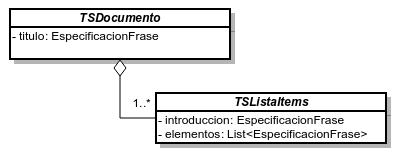
\includegraphics[scale=0.7]{img/text_spec.png}
	\caption{Text Specification.}
  	\label{fig:text_spec}
\end{figure}

Luego en la etapa de \emph{realización de estructura} se deberán transformar estas estructuras en anotaciones para el sistema de presentación.

En la literatura sobre NLG Podemos encontrar muchas alternativas en lo que respecta a la especificación de frases. Todas estas varían en el nivel de abstracción que tienen. Las representaciones mas abstractas le darán mas flexibilidad a las etapas de document planning y microplanning, pero al mismo tiempo nos obligarán a tener un realizador de superficie mas sofisticado. Por otro lado, las especificaciones menos abstractas, requieren que el document planner y el microplanner realicen un mayor trabajo, pero también tendrán mas control sobre el texto a producir. Uno de los objetivos que tuvimos a la hora de idear una estructura para nuestra especificación de frases fue que ésta sea independiente de nuestro problema, pretendemos que hable en términos del lenguaje que queremos generar y no en términos específicos de Z en nuestro caso. De esta forma podremos implementar un realizador de superficie que sea independiente de este problema y que pueda ser reutilizado. %TODO nota sobra la falta de un realizador en español al momento de desarrollar el trabajo


Es por esto que decidimos especificar las oraciones a generar mediante árboles sintácticos, donde los constituyentes de éstos serán los sintagmas\footnote{Grupo de palabras que ejercen una función sintáctica dentro de una oración} de la oración. Esto le dará la posibilidad al realizador lingüístico de poder identificar la función de cada uno de los constituyentes de la oración y poder trabajar por por ejemplo con el núcleo de un sintagma particular, debido a que, como vimos en el capítulo~\ref{sec:corpus_analisis}, necesitará conocer el núcleo del sujeto y el verbo de una oración para poder asegurarse de que haya concordancia de número y persona entre el verbo y el sujeto. 

En la figura~\ref{fig:phase_spec} podemos ver los elementos que utilizamos para modelar las frases de nuestro sistema.

\begin{figure}[H]
  	\centering
	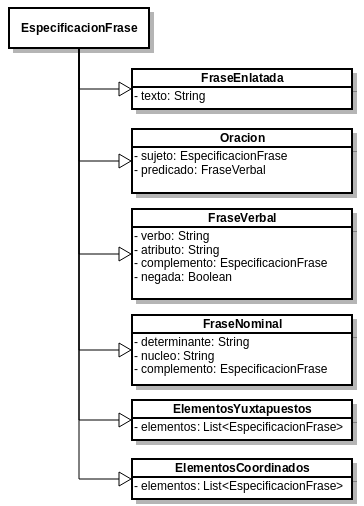
\includegraphics[scale=0.7]{img/phrase_spec.png}
	\caption{Phrase Specification.}
  	\label{fig:phase_spec}
\end{figure}

Como podemos observar no pretendemos modelar todo el lenguaje sino solo un subconjunto del mismo que provea las herramientas necesarias al realizador para generar las frases definidas en el capítulo~\ref{sec:corpus_analisis}, ya que el desarrollo de un realizador lingüístico que tenga en cuenta todas las construcciones de nuestro lenguaje escapa el alcance de nuestro trabajo. 

Es por esto que sólo modelaremos los sintagmas nominales (\emph{FraseNominal}) y verbales (\emph{FraseVerbal}) y nos veremos obligados a incluir otros elementos como \emph{ElementosYuxtapuestos} para salvaguardar la falta de algunos constituyentes sintácticos como sintagmas adjetivales, preposicionales, etc. 

A continuación describiremos brevemente cada uno de estos elementos, profundizando mas en detalle sobre la realización de los mismos en el capítulo~\ref{cap:linguistic_realization}.


\medskip
\begin{itemize}
\item{\emph{\textbf{FraseEnlatada}}: Representa texto que no necesita ningún tipo de procesamiento posterior a realizar durante la realización lingüística, será incluido en el texto tal cual fue establecido.}
\item{\emph{\textbf{Oracion}}: Modela oraciones bimembres. El realizador lingüístico deberá procesarlas en base a una serie de reglas gramaticales para producir un texto sintáctica, morfológica y ortográficamente correcto para éstas.}
\item{\emph{\textbf{FraseVerbal}}: Representa un sintagma verbal que corresponderá al predicado de una \emph{Oracion}.}
\item{\emph{\textbf{FraseNominal}}: Modela un sintagma nominal. Generalmente conformará el sujeto en una \emph{Oracion}.}
\item{\emph{\textbf{ElementosCoordinados}}: Representa una serie de elementos que se deberán transformar en una conjunción de frases en la etapa de realización lingüística, por ejemplo: \emph{``frase1\textbf{,} frase2 \textbf{y} frase3''}}
\item{\emph{\textbf{ElementosYuxtapuestos}}: Representa una lista ordenada de elementos que deberán ser realizados y \emph{concatenados} uno al lado del otro en la oración final. Nos vimos obligados a introducir este tipo de elementos para salvaguardar la falta de algunos constituyentes sintácticos como sintagmas adjetivales, preposicionales, etc.}
\end{itemize}


%\section{Arquitectura}

\section{Lexicalización}
\label{sec:microplanning_lexicalization}

Como mencionamos anteriormente, el proceso de lexicalización será el encargado de elegir que palabras particulares y constructores sintácticos usar para comunicar la información contenida en el document plan. En esta etapa deberemos producir una especificación de frase para cada mensaje contenido en el document plan. En nuestro caso debemos hacerlo utilizando como especificación el conjunto de reglas definidas anteriormente en base al \emph{corpus} en el capítulo~\ref{sec:corpus_analisis}.


El módulo encargado de esta tarea en nuestro sistema deberá ser capaz de generar una especificación de frase a partir de la expresión Z contenida en un mensaje del document plan. Primero deberá verificar si la expresión en cuestión se encuentra designada, en este caso, deberá construir una especificación de frase en base a su designación. De lo contrario deberá intentar construirla recursivamente de acuerdo a las reglas antes mencionadas. En la figura~\ref{fig:algoritmo_lexicalizacion} podemos ver un bosquejo del algoritmo del comportamiento que deseamos que tenga nuestro sistema. Este ejemplo es sólo para ilustrar el comportamiento deseado durante esta etapa. El algoritmo real resulta un poco más complejo y deberá construir una \emph{EspecificacionFrase} construyendo y componiendo sintagmas y otros de los elementos definidos en lugar del texto que vemos en el ejemplo. 

%TODO ver de cambiar esto por una parte del algoritmo posta
\begin{algorithm}[H]
\caption{Bosquejo Lexicalización.}
\begin{algorithmic}
\Function {lexicalizacion}{$exp$}
\If{$esta\_designada(exp)$}
\State $ret\gets \text{designacion}(exp)$
\Else
\State $ret\gets \text{lexicalizacion'}(exp)$
\EndIf
\State \textbf{return} $ret$
\EndFunction
\Statex
\Function {lexicalizacion'}{$\{x\} = y$}
\State $lexx\gets \text{lexicalizacion}(x)$
\State $lexy\gets \text{lexicalizacion}(y)$
\State \textbf{return} $\text{concat}(lexx, $\emph{``es el único elemento de''}$, lexxy)$
\EndFunction
\Statex
\Function {lexicalizacion'}{$x = y$}
\State $lexx\gets \text{lexicalizacion}(x)$
\State $lexy\gets \text{lexicalizacion}(y)$
\State \textbf{return} $\text{concat}(lexx, \text{\emph{``es(son) igual(es) a''}}, lexxy)$
\EndFunction
\Statex
\ldots
\end{algorithmic}
\label{fig:algoritmo_lexicalizacion}
\end{algorithm}

\begin{comment}
\Statex
\Function {lexicalizacion'}{$x = \{\}$}
\State $lexx\gets lexicalizacion(x)$
\State \textbf{return} $concat($\emph{``no hay elementos en''}$, lexx)$
\EndFunction

\begin{figure}[H]
\begin{verbatim}
lexicalizacion exp = if estaDesignada exp 
                     then designacion exp 
                     else lexicalizacion' exp

lexicalizacion' {x} \eq y  = lexicalizacion x ++
                             "es el único elemento de" ++
                             lexicalizacion y
lexicalizacion'  x  \eq {} = "no hay elementos en" ++
                             lexicalizacion y
lexicalizacion'  x  \eq y  = lexicalizacion x ++
                             "es(son) igual(es) a" ++
                             lexicalizacion y
...
\end{verbatim}
\label{fig:algoritmo_lexicalizacion}
\end{figure}
\end{comment}

La función \emph{designacion} deberá ser capaz de construir una especificación de frase a partir de una expresión designada\footnote{Escribimos esta función de esta forma para simplificar, pero la implementación de la misma es un poco mas compleja en realidad. Además de la expresión deberíamos saber el nombre del esquema al que pertenece la expresión ya que podría tratarse de una variable de esquema por ejemplo. Otro caso particular es el de las designaciones parametrizadas en el que deberá resolverse la designación del argumento primero para luego construir la designación pretendida.}. Para esto deberá recuperar el texto de esta designación y procesarlo a fin de crear una especificación de frase. Es razonable suponer que el texto de una designación sea un sintagma nominal, es decir tenga la siguiente estructura:


\begin{figure}[H]
  \centering
   Sintagma Nominal = [Determinante] + Núcleo + [Complemento]
\end{figure}

Por lo tanto nuestro sistema deberá trabajar el texto de las designaciones (haciendo uso de algún analizador morfológico) para construir una \emph{FraseNominal} a partir de cada designación. 

Por otro lado, en el caso que la expresión a lexicalizar no se encuentre designada, se deberá analizar recursivamente la expresión para generar el texto adecuado según las reglas antes mencionadas. 

Creemos que describir detalladamente nuestro algoritmo de lexicalización puede resultar muy engorroso para el lector debido a la cantidad de casos que debemos detallar (uno por cara regla de las antes mencionadas) y lo complejas que pueden resultar las especificaciones de frase. Es por esto que ilustraremos el resultado de nuestra lexicalización mediante un pequeño ejemplo.

Tomaremos como ejemplo el primer mensaje del el document plan de la figura~\ref{fig:png_document_plan_ej}. Nuestra misión será lexicalizar la expresión:

\begin{center}
$s? \in \dom st$
\end{center}

\noindent
contando con las siguientes designaciones:

\begin{align*} 
  &s? && \approx \text{el símbolo a buscar} \\
  &dom~x && \approx \text{símbolos cargados en la tabla de símbolos}
\end{align*}

En una primer instancia, al no encontrarse designada $s? \in \dom st$ nuestro lexicalizador deberá construir una \emph{Oracion} para la frase:

\begin{center}
lexicalizacion $s?$ ++ ``pertenece a'' ++ lexicalizacion $\dom st$ 
\end{center}

Para esto deberá resolver recursivamente la lexicalizacion de $s?$ y de $\dom st$ para formar el \emph{sujeto} y \emph{predicado} necesarios para la oración. Luego deberá formar una \emph{FraseVerbal} completando tanto el \emph{verbo} como el \emph{complemento} a fin de obtener el texto ``pertenece a'' en el texto final. En la figura~\ref{fig:phase_spec_ej} podemos observar el resultado final de la lexicalización.

\begin{figure}[H]
  	\centering
	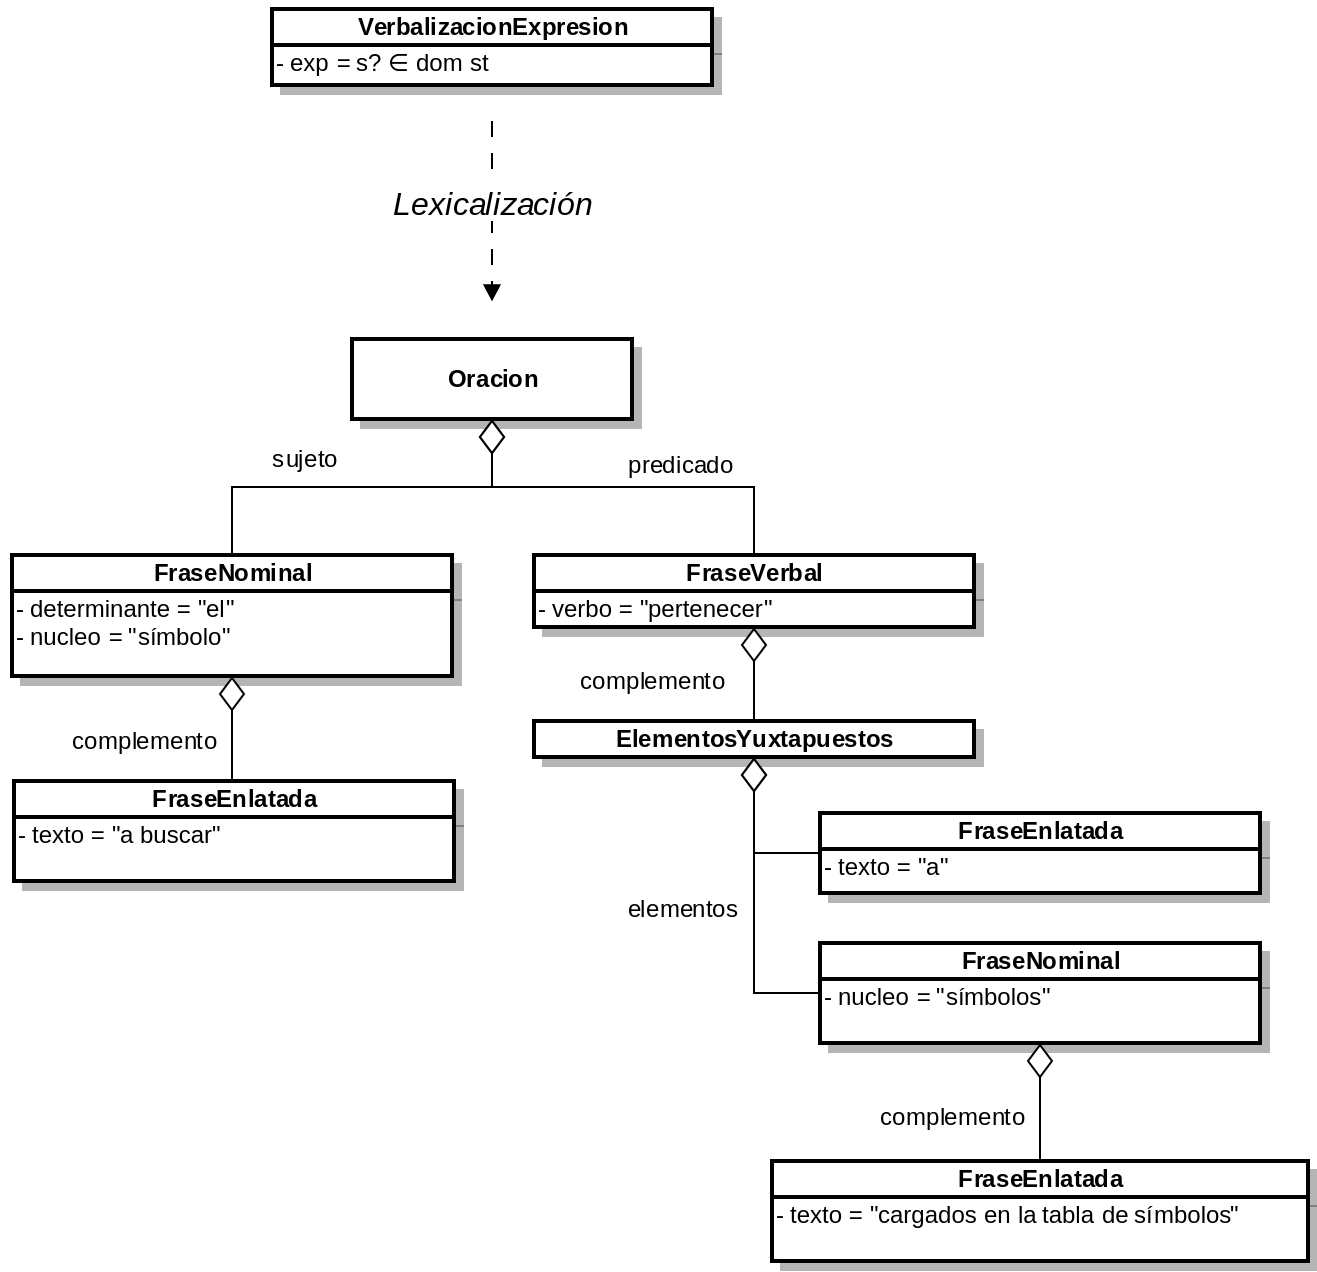
\includegraphics[scale=0.5]{img/phrase_spec_ej.png}
	\caption{Phrase Specification para.}
  	\label{fig:phase_spec_ej}
\end{figure}

Cabe aclarar que estableceremos el verbo en infinitivo siendo luego el realizador lingüístico el encargado de conjugar el mismo de acuerdo a algunas reglas gramaticales que veremos en el capítulo~\ref{cap:linguistic_realization}. Otra cuestión a mencionar es el uso del elemento \emph{ElementoYuxtapuestos} para salvaguardar la falta de un elemento que nos sirva para modelar un sintagma preposicional en este caso. Nuestro realizador lingüístico procesará los elementos contenidos en cada \emph{ElementoYuxtapuestos} generando un texto resultado de la concatenación de la realización los mismos.